\documentclass[runningheads]{llncs}

\usepackage[T1]{fontenc}
\usepackage{array}
\usepackage{booktabs}
\usepackage{longtable}
\usepackage{pgfplots}
\usepackage{url}

\pgfplotsset{compat=1.18}

\newcommand{\twolinecol}[2]{\texttt{#1}\newline\texttt{#2}}

\title{Deprecated KNIME Nodes in Source Repositories and User Workflows}
\titlerunning{Deprecated KNIME Nodes in Repositories and Workflows}

\author{Vitalii Kaplan\orcidID{0009-0009-8181-2863}}
\authorrunning{V. Kaplan}
\institute{\email{2333275007@alu.istinye.edu.tr}}

\begin{document}
\maketitle

\begin{abstract}
This study quantitatively analyzed deprecated functionality in visual
workflows as represented in KNIME's open-source code repositories and retained
in collected workflow examples. We found that deprecated
nodes are not a marginal phenomenon either on the KNIME platform or in
workflows created by KNIME users. We
reconstructed 13 source-date snapshots of the public \texttt{knime-oss}
repositories between April 2018 and June 2026 and parsed their structured
extension and compatibility metadata. Across these snapshots, the number of
deprecated nodes increased from 193 of 1301 (14.83\%) in the 2018
baseline to 502 of 1506 (33.33\%) in the latest snapshot. In addition, using the
latest snapshot, we built a deprecated-node registry and joined its factory-class
identifiers to 2745 node occurrences in 62 workflows uploaded by users to
k2pweb.org between 2026-03-25 and 2026-07-15. We found that 294 of the 2745 node
occurrences (10.71\%) were deprecated and that 21 of the 62 workflows (33.87\%)
contained at least one deprecated node.
This study is important because visual workflows
depend on evolving platform components, and deprecation can complicate their
later reuse and reproduction.

\keywords{KNIME \and Deprecated nodes \and Workflow reproducibility \and
Software evolution \and Repository mining}
\end{abstract}

\section{Introduction}

Visual workflows are widely used to construct scientific data analyses because
they express multi-step procedures as inspectable graphs of connected
operations. When the executable workflow and its software context are
preserved, this representation can support inspection, reuse, and
reproducibility across scientific domains
\cite{Liew2017Workflows,Ludascher2009Automation,Fu2025GIScienceKNIME,KaplanKNIMEWorkflowAudit2026}.

KNIME is one of the most widely used open-source visual workflow platforms in
scientific research. It represents data-analysis workflows as connected
processing nodes and has supported an extensible ecosystem since its early
platform description \cite{Berthold2009KNIME,KNIMEUserGuide2026}. Its public
source history and explicit extension metadata make it a suitable platform for
studying how visual-workflow components evolve.

Like other actively developed software platforms, KNIME changes over time.
Components can be replaced, hidden, declared deprecated, or removed as APIs,
interfaces, and recommended analytical practices evolve. The workflow
representation stores node identities and configuration alongside graph
structure, but the ability to reuse an older workflow also depends on the
lifecycle of those nodes and their extensions
\cite{DeRoure2011Preservation,Belhajjame2011Substitute}. A node may remain
loadable after it disappears from the ordinary authoring interface, be mapped
to a newer implementation, require a migration rule, or eventually depend on
an extension that is difficult to recover.

Scientific studies that use KNIME do not always preserve this software context.
A reproducibility audit of 100 highly cited KNIME-matching studies found that
18 reported a KNIME version, 22 reported a downloadable or linked workflow, and
workflow artifacts or workflow directories were obtained for 18 records
\cite{KaplanKNIMEWorkflowAudit2026}. Previous research likewise shows that
workflow reuse depends on contextual records, execution environments, and
continued access to suitable software
\cite{Willoughby2017Documentation,Ghoshal2021ScienceCapsule}. Missing workflow
artifacts and version information make it harder to determine which node
implementations a study used and whether those components remain available.

KNIME explicitly represents node deprecation in its extension metadata. The
official node schema describes deprecated nodes as hidden from the node
repository while still being loaded in existing workflows
\cite{KNIMEWorkbenchNodeSchema2026}. Because such nodes can remain loadable,
deprecation does not imply immediate failure; instead, it marks a workflow's
dependence on a legacy component outside the recommended authoring surface.
Interpreting this compatibility-risk marker requires both platform-side
evidence that distinguishes deprecated nodes from hidden nodes, removed
identities, factory-class mappings, and migration rules, and demand-side
evidence of whether the affected factory classes still occur in workflows.

The open-source knime2py project and its k2pweb.org interface provide this
demand-side perspective. knime2py parses KNIME workflows, reconstructs their
nodes and connections, and generates Python scripts or Jupyter notebooks for
supported nodes together with machine-readable graph representations
\cite{KaplanKnime2py2026}. The web service accepts a minimal workflow bundle,
runs knime2py in an isolated container, and returns the generated code and
graph outputs \cite{K2PWeb2026}. Because the submitted workflow structures retain
factory-class identities, they complement the platform metadata with evidence
of which KNIME node types still occur in practice.

Bringing these two evidence sources together, this work aims to quantify how
common deprecated nodes are in public KNIME source repositories and in observed
user workflows. We examine how declared deprecation changes across source
snapshots, which additions, removals, and status transitions accompany that
change, and which nodes classified as deprecated in the latest retained
snapshot occur in k2pweb workflows.

To answer these questions, we reconstruct 13 source-date snapshots of the
public \texttt{knime-oss} repositories from 2018 to 2026 and parse structured
extension metadata for ordinary nodes, dynamic node sets, hidden and deprecated
states, factory-class mappings, and migration rules. We then build a registry
of deprecated factory classes from the latest snapshot and use full factory
identifiers to perform an exact join between this registry and 2745 node
occurrences in 62 workflows uploaded by users to k2pweb for conversion from
KNIME to Python between 2026-03-25 and 2026-07-15.

The main contribution of this study is quantitative evidence that deprecated nodes are not a
marginal phenomenon in KNIME. In the latest source snapshot, 502 of 1506
ordinary-node registrations are deprecated, representing 487 distinct factory
classes. In the k2pweb data, 21 distinct deprecated factory classes account for
294 of 2745 node occurrences and appear in 21 of 62 user-uploaded workflows.
These platform- and demand-side measurements are supported by a reproducible
structured-XML mining method, retained per-snapshot evidence, and exact factory-
class matching that keeps KNIME lifecycle status separate from knime2py
translation support.

\section{Literature Review}

Scientific workflows have long been used to structure complex computational
experiments as connected data-processing and analytical steps. Reviews of
workflow systems describe their role in managing heterogeneous applications,
computing platforms, and data resources \cite{Liew2017Workflows}, while earlier
work identifies design, enactment, provenance, monitoring, and reuse as central
parts of scientific workflow management \cite{Ludascher2009Automation}.
Scientific workflow environments can consequently improve the reusability and
maintenance of workflows and their components, as well as support provenance,
version comparison, and failure recovery \cite{Altintas2006Accelerating}.

Workflows are also research artifacts that encode scientific methods. The
myExperiment repository treated workflows and experiment plans as born-digital
scholarly objects to be shared, reused, and curated across communities
\cite{Goble2010MyExperiment}. An empirical study of that repository nevertheless
identified technical, contextual, social, and motivational barriers to
workflow sharing and reuse \cite{Procter2009Sharing}. Repository availability
alone therefore does not ensure that a workflow can later be understood or
executed.

Workflow definitions themselves evolve during scientific exploration.
VisTrails, for example, records action-based provenance so that researchers can
navigate earlier workflow versions and parameter settings
\cite{Freire2006Managing}. Computational reproducibility, however, depends on
more than a history of edits or a published description of an analysis.
Provenance research in visual analytics argues for preserving records of the
data, the analytical process, and the interpretation needed for later
inspection and reuse \cite{Walker2013ProveML}.

Preservation research describes \emph{workflow decay} as the loss of
executability caused by external changes to the resources and services on
which a workflow depends \cite{DeRoure2011Preservation}. Related work addresses
this problem by identifying substitute services for unavailable workflow
operations \cite{Belhajjame2011Substitute}. This literature is conceptually
relevant to deprecated nodes because both concern dependencies that evolve
outside the persisted workflow. It does not, however, imply that a deprecated
component has already failed or that every obsolete component has a suitable
replacement.

Successful reuse also requires sufficient workflow context. KNIME-specific
work shows that storing a workflow without documentation, parameters, metadata,
associated data, and suitable software may be insufficient for later reuse
\cite{Willoughby2017Documentation}. The Science Capsule framework similarly
captures execution environments, contextual records, workflow versions, and
lineage to support sharing and reproduction \cite{Ghoshal2021ScienceCapsule}.
Even when an executable artifact is available, its dependencies can prevent
reproduction: a large-scale study of biomedical Jupyter notebooks found
failures during dependency installation and re-execution
\cite{SamuelMietchen2024JupyterReproducibility}. Research on preserving
computational environments shows how packaging software and its dependencies
can improve mobility and repeatability \cite{Kurtzer2017Singularity}. For a
node-based platform, this requirement extends to the workflow file, platform
version, installed extensions, and the implementations referenced by persisted
node identities.

Within this broader context, KNIME has been presented as an extensible visual
data-analysis environment
since its early platform description \cite{Berthold2009KNIME}. Its extension
model allows additional functionality to be installed from update sites
\cite{KNIMEExtensions2026}. This extensibility supports a broad analytical
ecosystem, but it also means that persisted workflows depend on node factories,
extension availability, and platform compatibility metadata. Recent work has
used KNIME workflows to support replicable and reproducible research, showing
the importance of maintaining their executable structure over time
\cite{Fu2025GIScienceKNIME}.

The KNIME source schemas distinguish several related mechanisms. Ordinary node
registrations and dynamic node sets can be marked deprecated. Hidden nodes are
also excluded from normal repository presentation, but hidden status does not
carry the same deprecation meaning. Separately, KNIME defines extension points
for mapping old persisted factory-class names to new implementations and for
registering workflow-node migration rules
\cite{KNIMECoreClassMapperSchema2026,KNIMEMigrationRuleSchema2026}. These
mechanisms support compatibility, but neither a mapper nor a migration rule is
itself evidence that a node is deprecated.

This study treats deprecation, hidden status, factory removal, factory-class
mapping, migration, and translation support as separate lifecycle dimensions.
Deprecation status is derived only from declared KNIME metadata, while mapping
and knime2py support are recorded independently. The analysis across source
snapshots therefore reports metadata states and transitions without
interpreting any individual state as evidence of workflow failure.

\section{Data}

\subsection{KNIME snapshot analysis}

The retained dataset contains 13 source-date snapshots selected through two
complementary sampling schemes. Release-anchored dates represent important
points in the available KNIME Analytics Platform release history
(Table~\ref{tab:release-snapshots}). Regular calendar checkpoints provide a
consistent basis for comparing source metadata between those releases
(Table~\ref{tab:calendar-snapshots}).

\begin{table}
\centering
\caption{Release-anchored KNIME source snapshots.}
\label{tab:release-snapshots}
\small
\begin{tabular}{p{0.19\textwidth}p{0.20\textwidth}p{0.51\textwidth}}
\toprule
Source date & Platform context & Role in the dataset \\
\midrule
2018-04-03 & 3.5.3 & Earliest locally available product-tag context and
study baseline \\
2019-12-05 & 4.1.0 & Anchor for the KNIME 4 release period \\
2023-02-22 & 5.0.0 & Anchor for the transition to KNIME 5 \\
2026-03-03 & 5.11.0 & Recent release anchor preceding the final study
checkpoint \\
\bottomrule
\end{tabular}
\end{table}

\begin{table}
\centering
\caption{Year-based and final-observation KNIME source snapshots.}
\label{tab:calendar-snapshots}
\small
\begin{tabular}{p{0.23\textwidth}p{0.67\textwidth}}
\toprule
Source date & Role in the dataset \\
\midrule
2019-01-01 & Annual checkpoint \\
2020-01-01 & Annual checkpoint \\
2021-01-01 & Annual checkpoint \\
2022-01-01 & Annual checkpoint \\
2023-01-01 & Annual checkpoint \\
2024-01-01 & Annual checkpoint \\
2025-01-01 & Annual checkpoint \\
2026-01-01 & Annual checkpoint \\
2026-06-28 & Final observation checkpoint \\
\bottomrule
\end{tabular}
\end{table}

Each row represents the state of the retained public source repositories at
the specified date. Release anchors therefore provide version context, whereas
the January checkpoints provide regular comparison intervals. The final
2026-06-28 row captures the latest source state included in the study. These
snapshots are reconstructed source states rather than archived binary KNIME
distributions.

The original snapshot evidence is stored under:
\begin{quote}
\path{data/original/knime_snapshots/}
\end{quote}
The processed table is:
\begin{quote}
\path{data/processed/knime_snapshots/}\\
\path{knime_node_snapshot_summary.csv}
\end{quote}
Its main measurement groups are shown in Table~\ref{tab:summary-columns}.

\begin{table}
\centering
\caption{Main measurement groups in the processed snapshot summary.}
\label{tab:summary-columns}
\small
\begin{tabular}{p{0.31\textwidth}p{0.60\textwidth}}
\toprule
Group & Measurements \\
\midrule
Snapshot provenance & Identifier, date, source basis, version context,
processed and skipped repositories \\
Node registrations & Ordinary nodes, dynamic node sets, total registrations,
and unique factory classes \\
Deprecation & Deprecated ordinary nodes and node sets, unique deprecated factory
classes, and deprecated share \\
Related states & Hidden nodes, nodes both deprecated and hidden, and deprecated
node descriptions \\
Compatibility metadata & Factory-class mapper and migration-rule contribution
counts \\
Adjacent transitions & Added, removed, newly deprecated, no longer deprecated,
newly hidden, no longer hidden, and category-changed identities \\
\bottomrule
\end{tabular}
\end{table}

The number of repositories available at early dates is smaller because some
repositories did not yet exist. Checkout manifests preserve this changing
coverage. The processed table is derived evidence; the per-record XML
extractions and checkout manifests remain authoritative for auditing individual
counts.

\subsection{Deprecated-node usage}

k2pweb.org is an online service for converting KNIME workflows into executable
Python representations \cite{K2PWeb2026}. A user uploads a KNIME workflow to
the service and receives generated Python code, including scripts or Jupyter
notebooks that can be downloaded and executed. The service performs the
conversion by running the open-source knime2py converter
\cite{KaplanKnime2py2026}.

The study team had authorized access to the k2pweb.org database and therefore
exported structural records from the workflows submitted for
conversion. The export used in this study was downloaded on 2026-07-15 and
covers workflows recorded from the k2pweb release on 2026-03-25 through the
download date. The retained file contains workflow-local identifiers and node
factory classes rather than uploaded workflow contents or user identifiers. It
is stored in:
\begin{quote}
\path{data/original/k2pweb/factories.csv}
\end{quote}
The file contains 2745 node-occurrence records from 62 workflows
and includes 160 distinct fully qualified factory classes. Each value in the
\texttt{index} column uniquely identifies one workflow within the
export. Each value in the \texttt{factory} column is the fully qualified KNIME
node factory class for one node occurrence. Consequently, repeated rows for a
factory within the same workflow represent multiple occurrences of that node
type, rather than duplicate workflow records. The file contains no workflow
contents, node settings, user identifiers, or session identifiers.

This original file records node usage, not KNIME lifecycle status. Deprecated
usage is determined by joining the full \texttt{factory} value to the KNIME
source metadata using exact identifiers. Results for workflow prevalence,
occurrence prevalence, distinct node types, and unmatched identifiers are
reported separately; no suffix or partial-string match is treated as evidence of
deprecation.

The processed artifacts are a registry of unique deprecated factory classes in
the 2026-06-28 snapshot, an audit table retaining the join outcome for every
observed factory class, and an aggregate usage summary:
\begin{quote}
\path{data/processed/k2pweb/}\\
\path{deprecated_node_factory_registry.csv}\\
\path{k2pweb_factory_join_audit.csv}\\
\path{k2pweb_deprecated_node_usage_summary.csv}
\end{quote}

\section{Methods}

\subsection{KNIME snapshot analysis}

We mine the public \texttt{knime-oss} repositories using date-based source
snapshots. The local clone contains 91 top-level Git repositories. The mining
process includes 90 non-hidden repositories and excludes the organization-level
\texttt{.github} repository. For each target date, every included repository is
checked out to its latest commit at or before 23:59:59 on that date. The
checkout script is stored as:
\begin{quote}
\path{scripts/knime_source/}\\
\path{checkout_knime_oss_by_date.sh}
\end{quote}
It writes a manifest containing the repository, checkout status, target date,
selected commit and commit date, and previous HEAD.

For each reconstructed snapshot, \path{scripts/knime_source/collect_knime_node_snapshot.py}
parses structured XML rather than searching source text. It skips
\texttt{.git}, \texttt{target}, \texttt{bin}, and \texttt{.metadata}
directories. Boolean XML attributes are true only when their values are
case-insensitively equal to \texttt{true}.

The primary ordinary-node deprecation marker is
\texttt{deprecated="true"} under the Eclipse extension point:

\begin{quote}
\texttt{org.knime.workbench.repository.nodes}
\end{quote}

Dynamic node sets are collected separately from:

\begin{quote}
\texttt{org.knime.workbench.repository.nodesets}
\end{quote}

XML files whose names end in \texttt{NodeFactory.xml} and whose root element is
\texttt{knimeNode} are parsed as a secondary description-level source. Ordinary
registrations whose \texttt{hidden} attribute is true are counted separately
from deprecated registrations. The extractor also records contributions to the
following extension points:
\begin{quote}
\path{org.knime.core.NodeFactoryClassMapper}\\
\path{org.knime.workflow.migration.NodeMigrationRule}
\end{quote}
These records describe compatibility mechanisms and are not counted as
deprecation markers.

The per-snapshot outputs are:

\begin{itemize}
\item \path{logs/checkout_<snapshot-date>.csv};
\item \path{plugin_nodes.csv};
\item \path{node_descriptions.csv};
\item \path{factory_class_mappers.csv};
\item \path{migration_rules.csv}; and
\item \path{summary.csv}.
\end{itemize}

The summary builder is stored under \path{scripts/knime_source/} as
\path{build_knime_node_snapshot_summary.py}. It orders snapshots and calculates
aggregate counts. It also compares adjacent snapshots. A non-empty factory
class is used as the node identity. Registrations without one use the fallback
key \path{plugin_xml:element:category_path}. Added and removed identities are
set differences. Transitions in deprecation status, hidden status, and category
are calculated only for identities present in both adjacent snapshots. These are
metadata-level approximations because refactoring a factory class can change
the observed identity.

\subsection{Deprecated-node usage}

The usage-analysis script is stored as:
\begin{quote}
\path{scripts/k2pweb/}\\
\path{build_deprecated_node_usage.py}
\end{quote}
It builds the deprecated-node factory registry from ordinary \texttt{node}
registrations in the 2026-06-28 snapshot. A factory enters the registry when at
least one of its registrations has a \texttt{deprecated} value that is
case-insensitively equal to \texttt{true}.
Multiple registrations of the same full factory class are aggregated into one
registry row while retaining registration counts, repositories, plug-in XML
files, category paths, and hidden-registration counts.

The script then joins each k2pweb \texttt{factory} value to the complete set of
ordinary-node factory classes in that snapshot. Exact matches are classified as
deprecated or not deprecated; identifiers absent from the snapshot are retained
as \texttt{not\_found}. No partial-string, suffix, or inferred-alias match is used.
The analysis reports exact-join coverage before deprecation prevalence and
uses workflows, node occurrences, and distinct factory classes as
separate denominators. A workflow is classified as containing deprecated usage
when at least one of its occurrences exactly matches a registry factory.

\section{Results}

\subsection{KNIME snapshot analysis}

This subsection reports how declared ordinary-node deprecation changes across
the retained KNIME source snapshots. It first presents the percentage trend at
the annual checkpoints and then examines selected release anchors, repository
coverage, and changes between adjacent snapshots. All percentages use
registered ordinary nodes as the denominator; dynamic node sets are reported
separately. Figure~\ref{fig:deprecated-percent-year} shows the annual trend,
using the 2018-04-03 baseline for 2018 and the January checkpoint for each year
from 2019 through 2026.

\begin{figure}
\centering
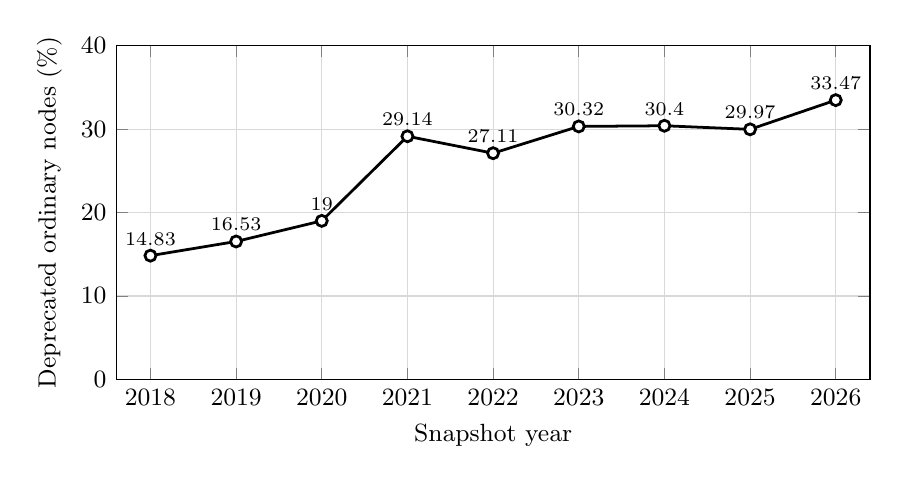
\begin{tikzpicture}
\begin{axis}[
  width=0.92\textwidth,
  height=0.48\textwidth,
  xlabel={Snapshot year},
  ylabel={Deprecated ordinary nodes (\%)},
  xmin=2017.6,
  xmax=2026.4,
  ymin=0,
  ymax=40,
  xtick={2018,2019,2020,2021,2022,2023,2024,2025,2026},
  xticklabel style={/pgf/number format/1000 sep={}},
  ytick={0,10,20,30,40},
  grid=major,
  major grid style={draw=gray!30},
  tick label style={font=\small},
  label style={font=\small},
  nodes near coords,
  every node near coord/.append style={font=\scriptsize,anchor=south},
  point meta={y},
  scaled ticks=false
]
\addplot[
  color=black,
  mark=*,
  mark options={fill=white},
  line width=1pt
] coordinates {
  (2018,14.83)
  (2019,16.53)
  (2020,19.00)
  (2021,29.14)
  (2022,27.11)
  (2023,30.32)
  (2024,30.40)
  (2025,29.97)
  (2026,33.47)
};
\end{axis}
\end{tikzpicture}
\caption{Percentage of registered ordinary KNIME nodes marked deprecated at
the annual source checkpoints. The 2018 point uses the earliest retained
baseline of 2018-04-03; subsequent points use January 1 snapshots.}
\label{fig:deprecated-percent-year}
\end{figure}

At the earliest source baseline, 2018-04-03, 193 of 1301 registered ordinary
nodes were marked deprecated, or 14.83\% (Table~\ref{tab:selected-snapshots}).
At the KNIME Analytics Platform 5.0.0 source-date anchor on 2023-02-22, the
count is 433 of 1442 nodes, or 30.03\%. The final 2026-06-28 snapshot contains
502 deprecated ordinary nodes out of 1506, or 33.33\%. The declared share of
deprecated nodes therefore approximately doubles between the earliest and
final retained snapshots.

\begin{table}
\centering
\caption{Selected KNIME repository-mining snapshots.}
\label{tab:selected-snapshots}
\scriptsize
\begin{tabular}{lp{0.34\textwidth}rrr}
\toprule
Date & Version context & Nodes & Deprecated & Share \\
\midrule
2018-04-03 & Analytics Platform 3.5.3 source-date anchor & 1301 & 193 & 14.83\% \\
2019-12-05 & Analytics Platform 4.1.0 source-date anchor & 1191 & 227 & 19.06\% \\
2023-02-22 & Analytics Platform 5.0.0 source-date anchor & 1442 & 433 & 30.03\% \\
2026-03-03 & Analytics Platform 5.11.0 source-date anchor & 1503 & 503 & 33.47\% \\
2026-06-28 & Current local source-date snapshot & 1506 & 502 & 33.33\% \\
\bottomrule
\end{tabular}
\end{table}

Annual checkpoints show the same broad increase while making the changing
repository coverage explicit (Table~\ref{tab:annual-snapshots}). The number of
repositories with a valid checkout rises from 44 in 2018 to 90 in 2026, so raw
early and late node totals do not describe a fixed source corpus. The deprecated
share is less sensitive to this difference but can still be affected by
repositories entering the corpus. Hidden ordinary nodes remain much less
frequent, increasing from 2
in the 2018 checkpoint to 24 in 2026. Deprecated dynamic node sets appear from
2020 onward and remain at 2 through the 2026 annual checkpoint.

\begin{table}
\centering
\caption{Annual KNIME repository-mining checkpoint statistics.}
\label{tab:annual-snapshots}
\scriptsize
\begin{tabular}{llrrrrrr}
\toprule
Year & Date & Repos & Nodes & Deprecated & Node sets & Hidden & Share \\
\midrule
2018 & 2018-04-03 & 44 & 1301 & 193 & 0 & 2 & 14.83\% \\
2019 & 2019-01-01 & 45 & 1500 & 248 & 0 & 2 & 16.53\% \\
2020 & 2020-01-01 & 54 & 1200 & 228 & 2 & 2 & 19.00\% \\
2021 & 2021-01-01 & 60 & 1366 & 398 & 2 & 5 & 29.14\% \\
2022 & 2022-01-01 & 67 & 1424 & 386 & 2 & 8 & 27.11\% \\
2023 & 2023-01-01 & 72 & 1428 & 433 & 2 & 10 & 30.32\% \\
2024 & 2024-01-01 & 80 & 1434 & 436 & 2 & 9 & 30.40\% \\
2025 & 2025-01-01 & 86 & 1488 & 446 & 2 & 23 & 29.97\% \\
2026 & 2026-01-01 & 90 & 1509 & 505 & 2 & 24 & 33.47\% \\
\bottomrule
\end{tabular}
\end{table}

The transition results show bursts rather than a constant deprecation rate
(Table~\ref{tab:annual-transitions}). The largest annual counts of common node
identities newly marked as deprecated occur in 2021, 2023, and 2026: 80, 61, and
60, respectively. The 2022 checkpoint is the only annual row with a substantial
count of common identities no longer marked deprecated (29). Category-path
changes are concentrated in 2021 and 2023.

\begin{table}
\centering
\caption{Annual adjacent-snapshot transition statistics.}
\label{tab:annual-transitions}
\scriptsize
\begin{tabular}{lrrrrr}
\toprule
Year & Added & Removed & Newly deprecated & No longer deprecated & Category changed \\
\midrule
2018 & -- & -- & -- & -- & -- \\
2019 & 194 & 22 & 16 & 0 & 6 \\
2020 & 11 & 0 & 0 & 0 & 4 \\
2021 & 140 & 1 & 80 & 0 & 111 \\
2022 & 69 & 6 & 17 & 29 & 17 \\
2023 & 56 & 4 & 61 & 0 & 67 \\
2024 & 17 & 7 & 4 & 0 & 3 \\
2025 & 36 & 0 & 9 & 0 & 1 \\
2026 & 52 & 2 & 60 & 0 & 3 \\
\bottomrule
\end{tabular}
\end{table}

These snapshot results measure declared source metadata, not workflow
execution. Taken alone, they do not establish usage frequency, whether a
particular deprecated node still runs, or whether deprecation caused a
translation failure. They establish that deprecation is a substantial and
changing part of the public KNIME node surface and provide the classification
registry for the demand-side analysis below.

\subsection{Deprecated-node usage}

This subsection quantifies the presence of deprecated nodes in workflows
submitted to k2pweb for conversion. It first establishes the deprecated-factory
registry and exact-identifier join coverage, then examines unmatched factory
classes and reports deprecated-node prevalence at the workflow, node-occurrence,
and distinct-factory levels.

The 2026-06-28 registry contains 487 unique deprecated factory classes derived
from 502 deprecated ordinary-node registrations. Fifteen factory classes have
two deprecated registrations each. This explains the difference between the
factory- and registration-level counts.

Exact matching links 146 of the 160 factory classes observed in k2pweb
(91.25\%) to ordinary-node factory classes in the classification snapshot.
These matches account for 2549 of 2745 occurrences (92.86\%). The remaining 14
factory classes and 196
occurrences are unmatched because their exact factory identifiers do not occur
among the ordinary-node registrations in the 2026-06-28 classification
snapshot. They are therefore retained in the join audit but excluded from
claims about their deprecation state.

The unmatched identifiers have more than one explanation. The factory
\path{org.knime.dynamic.js.v30.DynamicJSNodeFactory} is produced dynamically by
\path{DynamicJSNodeSetFactory}; it is therefore not represented as an ordinary
\texttt{node} registration and cannot match the ordinary-node registry. The
factory
{\scriptsize\path{org.knime.timeseries.node.stringtotimestamp.String2DateNodeFactory}}
appears as an ordinary registration in the 2018 and 2019 snapshots but is absent
from the later retained snapshots. Older persisted workflows can nevertheless
retain its factory identifier. The remaining 12 unmatched factory classes never
appear as ordinary registrations in any retained public source snapshot. They
may originate from separately distributed extensions, non-public distribution
bundles, or components outside the included \texttt{knime-oss} repositories.
This group comprises JEP, Data Generation, Tableau, Formulas, and newer
base-view factories.

Among all 62 workflows, 21 contain at least one exact match to a
deprecated factory (33.87\%). Deprecated factories account for 294 of 2745
node occurrences (10.71\%) and 21 distinct observed factory classes.
Table~\ref{tab:k2pweb-usage} keeps the three counting units separate.

\begin{table}
\centering
\caption{Exact-join coverage and deprecated-node usage in k2pweb.}
\label{tab:k2pweb-usage}
\small
\begin{tabular}{lrrr}
\toprule
Measurement & Count & Denominator & Share \\
\midrule
Exactly matched factory classes & 146 & 160 & 91.25\% \\
Exactly matched occurrences & 2549 & 2745 & 92.86\% \\
Workflows with deprecated usage & 21 & 62 & 33.87\% \\
Deprecated node occurrences & 294 & 2745 & 10.71\% \\
Distinct deprecated factory classes & 21 & 160 & 13.13\% \\
\bottomrule
\end{tabular}
\end{table}

These classifications show that nodes declared deprecated in the selected
source snapshot remain present in submitted workflows, but they do not
establish execution failure, translation failure, or causation.

\section{Discussion}

The main result is a growing declared legacy surface. Approximately one third
of registered ordinary nodes are deprecated in the latest retained snapshot,
compared with about one seventh at the earliest source baseline. This change is
not monotonic across the checkpoints, and it occurs alongside changing
repository coverage, node additions, removals, category changes, and compatibility
metadata. The per-snapshot records are therefore more informative than a single
current count.

Deprecation should be interpreted cautiously. KNIME deliberately loads
deprecated nodes in existing workflows, so the marker both supports backward
compatibility and signals risk. A deprecated workflow node may remain
fully executable. Conversely, a workflow may fail because of a missing
extension, input, configuration, or external dependency even when none of its
nodes is deprecated. Repository metadata can identify candidates for
compatibility inspection, but runtime claims require workflow-level testing.

The next repository-mining step is a node-level lifecycle table recording first
and last appearance, first deprecation, hidden status, removal from later
snapshots, category changes, and links to factory-class mapper or migration-rule
evidence. Manual validation should cover representative deprecated, hidden,
removed, migrated, and inconsistent records. This will distinguish persistent
low-risk legacy nodes from nodes with unclear migration paths.

The k2pweb analysis provides complementary demand-side evidence
\cite{KaplanKnime2py2026,K2PWeb2026}. One third of the observed workflows
contain a node classified as deprecated in the latest source snapshot, although
deprecated nodes form a smaller share of occurrences. This workflow sample is
self-selected and is not representative of all KNIME
workflows. Raw logs, uploaded workflows, settings, paths, credentials, IP
addresses, and stable user identifiers remain outside the research repository.
Future exports should add translation-support and conversion-outcome fields
without weakening this privacy boundary.

Finally, an association between deprecated-node presence and conversion failure
would remain descriptive unless the failure can be isolated to the affected
node. The stronger practical contribution is an evidence-backed advisory layer:
detect deprecated nodes, report their source-snapshot status, identify explicit
mapper or migration evidence, and warn when translation or repair requires
manual intervention.

\bibliographystyle{splncs04}
\bibliography{references}

\end{document}
